\documentclass[]{standalone}
\usepackage{tikz}
\usetikzlibrary{shapes,arrows,calc,positioning}
\usepackage{amsmath} % for dfrac

% definition of basic block
\tikzset{
    block/.style = {draw, rectangle,
        minimum height=1.2cm,
        minimum width=2cm},
    input/.style = {coordinate,node distance=1cm},
    output/.style = {coordinate,node distance=1cm},
    sum/.style = {draw, circle, node distance=1cm},
}

% definition of saturation block
\tikzset{% from https://tex.stackexchange.com/questions/161075/saturation-block
  saturation block/.style={%
    draw, 
    path picture={
      % Get the width and height of the path picture node
      \pgfpointdiff{\pgfpointanchor{path picture bounding box}{north east}}%
        {\pgfpointanchor{path picture bounding box}{south west}}
      \pgfgetlastxy\x\y
      % Scale the x and y vectors so that the range
      % -1 to 1 is slightly shorter than the size of the node
      \tikzset{x=\x*.4, y=\y*.4}
      %
      % Draw annotation
      \draw (-1,0) -- (1,0) (0,-1) -- (0,1); 
      \draw (-1,-.7) -- (-.6,-.7) -- (.6,.7) -- (1,.7);
    }
  }
}
\tikzset{% from https://tex.stackexchange.com/questions/161075/saturation-block
  deadband block/.style={%
    draw, 
    path picture={
      % Get the width and height of the path picture node
      \pgfpointdiff{\pgfpointanchor{path picture bounding box}{north east}}%
        {\pgfpointanchor{path picture bounding box}{south west}}
      \pgfgetlastxy\x\y
      % Scale the x and y vectors so that the range
      % -1 to 1 is slightly shorter than the size of the node
      \tikzset{x=\x*.4, y=\y*.4}
      %
      % Draw annotation
      \draw (-1,0) -- (1,0) (0,-1) -- (0,1);  % axis
      \draw (-1,1) -- (-.3,.3) -- (-.3,0) -- (.3,0) -- (.3,-.3) -- (1,-1);
	  %\draw (-.3,.3) -- (.3,-.3) ;
    }
  }
}
\begin{document}
	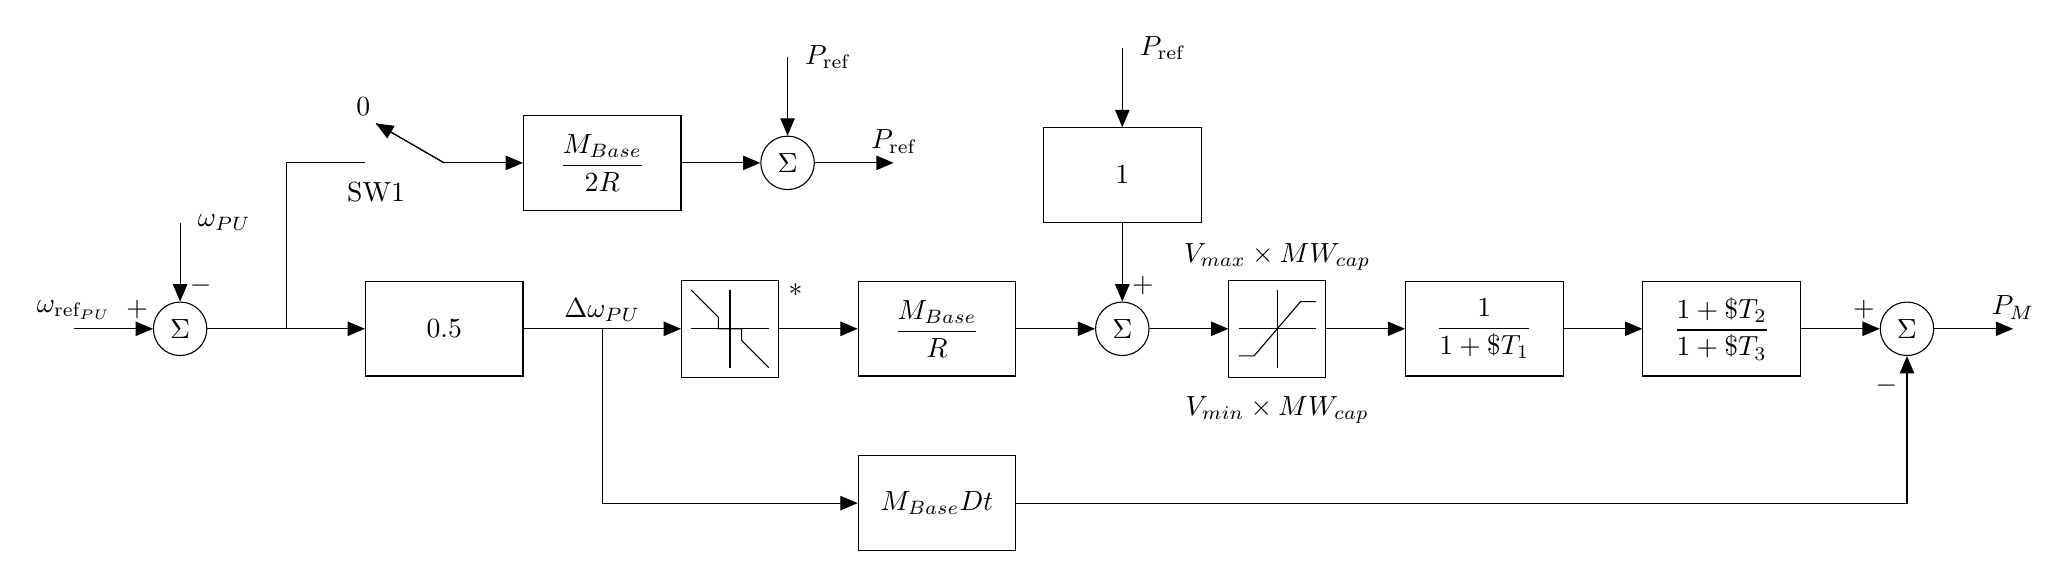
\begin{tikzpicture}[auto, node distance=1cm,>=triangle 45]
		% Starting input (wref)
		\node [input, name=input, label=$\omega_{\text{ref}_{PU}}$] {};
		% sum 1
		\node [sum, right=of input] (sum1) {$\Sigma$};
		
		% DTC junction
		\coordinate [right=of sum1]  (DTCw) {};
		% delay block w
		\node [block, right=of DTCw,label=17:] (delay1) {$0.5$};
		
		% delta w node and label
		\coordinate [right=of delay1]  (deltaw) {};
		\node [above=-.8em of deltaw,label={$\Delta\omega_{PU}$}]  (deltaWlabel){};
		
		% Hz Deadband
		\node [deadband block, right=of deltaw, minimum size=3.5em,label=17:*] (deadband) {};

		% DTC logic
		\node [block, above=1.5cm of deltaw] (DTClogic) {$\dfrac{M_{Base}}{2R}$};
		% sum DTC
		\node [sum, right=of DTClogic] (DTCsum) {$\Sigma$};

		\coordinate [left=of DTClogic]  (dtcSwithR) {};
		\coordinate [left=of dtcSwithR]  (dtcSwithL) {};

		\node [input, name=PrefDTCin, above= of DTCsum,label={[label distance=.1cm]0:$P_{\text{ref}}$} ] {};
		\node [output, right=of DTCsum, label=$P_{\text{ref}}$] (PrefOut) {};
		
		% delta w gain blocks
		\node [block, right=of deadband] (gain) {$\dfrac{M_{Base}}{R}$};
		\node [block, below=of gain] (Dt) {$M_{Base} Dt$};
		% Pref sum
		\node [sum, right=of gain] (sumP) {$\Sigma$};
		% delay block Pref
		\node [block, above=of sumP,label=17:] (delay2) {$1$};
		
		% limiter and labels
		\node [saturation block, right=of sumP , minimum size=3.5em, label=$V_{max} \times MW_{cap}$] (mwcap){};
		\node [below=2em of mwcap, label=$V_{min} \times MW_{cap}$](mwcapLOW){};
		% Valve state block
		\node [block, right=of mwcap] (state1) {$\dfrac{1}{1+\$T_1}$};
		% turbine state
		\node [block, right=of state1] (state2) {$\dfrac{1+\$T_2}{1+\$T_3}$};
		% damping sum
		\node [sum, right= of state2] (sum2) {$\Sigma$};
		% Pm out
		\node [output, right=of sum2, label=$P_M$] (output) {};
		% w and pref in
		\node [input, name=omega, above= of sum1,label={[label distance=.1cm]0:$\omega_{PU}$} ] {};
		\node [input, name=Pref, above= of delay2,label={[label distance=.1cm]0:$P_{\text{ref}}$} ] {};

		% connecting lines
		\draw [draw,->] (input) -- node[pos=0.8] {$+$} (sum1); % straight connecting line
		\draw [->] (omega) --  node[pos=0.8] {$-$} (sum1);
		\draw [->] (sum1) -- (delay1);
		\draw [->] (Pref) -- (delay2);
		\draw [->] (delay2) -- node[pos=0.8] {$+$} (sumP);
		\draw [->] (delay1) -- (deadband) ;
		\draw [->] (deadband) -- (gain) ;
		\draw [->] (gain) -- (sumP) ;
		\draw [->] (sumP) -- (mwcap) ;
		\draw [->] (mwcap) -- (state1) ;
		\draw [->] (state1) -- (state2) ;
		\draw [->] (state2) -- node[pos=0.8] {$+$} (sum2);
		\draw [->] (deltaw) |-  (Dt); % line goes down and across
		\draw [->] (Dt) -|  node[pos=0.9] {$-$} (sum2); % line goes across then down
		\draw [->] (sum2) -- (output);

		% DTC Lines
		\draw  (DTCw) |- (dtcSwithL) ;
		\draw  (dtcSwithR) -- ++(150:1) node (zeroIn) [label={[label distance=-.2cm]150:0}] {} ;
		\draw [->] (dtcSwithR) -- ++(150:1) node (SWlabel) [label={[label distance=.5cm]270:SW1}] {} ;
		\draw [->] (dtcSwithR) -- (DTClogic) ;
		\draw [->] (DTClogic) -- (DTCsum) ;
		\draw [->] (PrefDTCin) -- (DTCsum) ;
		\draw [->] (DTCsum) -- (PrefOut) ;
		
	\end{tikzpicture} 
\end{document}